
\section{Problems}
\label{problems}

\begin{enumerate}
\def\labelenumi{\arabic{enumi}.}
\item
  Why is it important for a model to separate the design of a system
  from its realization?

\item
  Classify each of the following as either a model, not a model, or
  sometimes a model. Justify your answer based on the definition and
  properties of a model.

\begin{itemize}
\def\labelenumi{\alph{enumi})}
\item Adiagram of a subway system,
\item a computer program, 
\item a football play, 
\item drivers license,
\item a floor plan of the local shopping mall (a ``you are here'' diagram)., 
\item an equation, 
\item A scratch n' sniff perfume advertisement in a fashion magazine,
\item The 1812 overture,
\item a braille sign reading ``second floor'',
\item sheet music for the Brandenburg Concerto, 
\item the United States Constitution, 
\item a set of car keys,
\item the ASCII encoding of an email message.
\end{itemize}


  \item
    Which of the following systems has memory? Justify your answer using
    the concepts of input, output, and state.
\begin{itemize}
\def\labelenumi{\alph{enumi})}
\item  an ink pen,
\item a resistor,
\item a capacitor,
\item a motorized garage door,
 \item an analog wrist watch, 
\item the air pressure in an air compressor, 
\item  the thermostat which controls the furnace in a house, 
\item a light switch, 
\item a political system,
\item the temperature of a large lake, 
\item  a book, 
\item a computer's hard drive.
\end{itemize}


  \item
    A can of soda has memory. Your objective is to figure out what
    characteristic of the can is the state variable and what input
    causes it to change. Based upon this, draw a state diagram for a can
    of soda. Label the transition arcs with the input responsible for
    the transition. Hint: no special equipment is needed to elicit the
    change of state.
  \item
    Consider the state diagram for the vending machine shown in Figure
    6.2. Now assume that the system accepts nickels, dimes, and
    quarters. Also assume that it is capable of returning change to the
    user after a purchase. Create a state diagram that represents this
    new system. Make sure to define the output signals and their value
    for each state.
  \item
    Use a state diagram to describe the high level operation of the
    ChipMunk Recorder (CMR). The CMR records sounds and then plays them
    back at a variety of speeds, making a recorded voice sound like a
    high pitched chipmunk. The CMR receives user input from a keyboard
    and an audio source. The behavior of the system is described as
    follows:

\begin{itemize}
\item
  When powered up, the CMR enters a wait state.
\item
  If \textquotesingle R\textquotesingle{} is pressed the recorder begins
  recording.
\item
  Any key-press will put the CMR back into the wait state.
\item
  If \textquotesingle S\textquotesingle{} is pressed, the CMR is ready
  to change the playback speed. A subsequent numerical input between 1
  and 5 will cause the playback speed to be changed to that value.
\item
  Pressing the \textquotesingle R\textquotesingle{} key when in the
  adjust playback speed mode will cause the CMR to go to the wait state.
\item
  Pressing a \textquotesingle P\textquotesingle{} key will cause the CMR
  to playback the recorded sounds. When done playing the entire
  recording, the CMR will loop back and start playing at the beginning.
\item
  Any key-press while in the playback mode will cause the CMR to go back
  into the wait state.
\end{itemize}

  Draw a state diagram describing the behavior of the CMR. Create a
  table which lists every state and its associated output.

  \item
    Build a state diagram to describe the state of the tape cartridges
    used to backup a company's network drives. When new
    \textbf{unformatted} cartridges are received they are immediately
    labeled with a unique ID. Before a tape is used it is formatted
    turning it into a \textbf{blank} tape. On the first day of the week
    a complete backup is made of the network drives, transforming blank
    tapes into \textbf{active} tapes. The active tapes, made every
    fourth week, are moved off site making them \textbf{archival} tapes.
    Active tapes older than 3 months are assumed to have out of date
    information and are reformatted into blank tapes. Archival tapes
    more than 2 years old are reformatted and put back into circulation.
  \item
    Build a flowchart to describe the operation of a microcontroller
    (MCU) based temperature regulating system. The system monitors the
    temperature of a heated environment using thermistors and regulates
    the temperature by turning fans on to cool the environment. The MCU
    periodically reads the temperature from each of the 64 different
    thermistors (each is driven by its own constant current source) by
    selecting each through an analog multiplexor. The voltage is
    converted into an 8-bit digital value using the MCU's
    analog-to-digital converter. If any of the 64 thermistors exceeds a
    high temperature threshold, the MCU uses a complex algorithm to
    determine the number of fans to turn on, otherwise all the fans are
    turned off.
  \item
    Write an algorithmic description for each of the flow charts below
    using while, if, or do statements.

\begin{tabular}{m{4cm}m{4cm}m{4cm}}
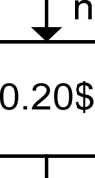
\includegraphics[width=1.4in,height=1.2in]{./image16} &
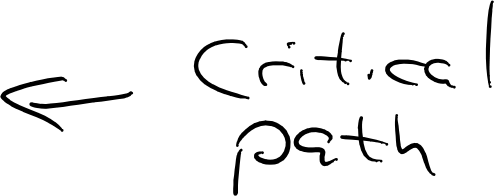
\includegraphics[width=0.83in,height=1.5in]{./image17} &
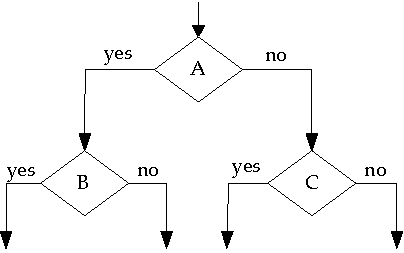
\includegraphics[width=2.4in,height=1.46in]{./image18} \\
(a) &  (b)  & (c) \\
\end{tabular}

\item
  Create a flowchart that outlines how to crochet a two-tone blanket
  with a diagonal stripe across it as shown below. A blanket is
  crocheted by linking together a sequence of basic stitches. For the
  purposes of the flowchart assume that a basic stitch is an elaborate
  process. Basic stitches are made from either dark or light yarn. The
  blanket should be 100 stitches wide by 150 stitches high. The diagonal
  stripe runs at a 45 degree angle from the horizontal.


\includegraphics[width=1in,height=1.34in]{./image19}


\item
  Build a data flow diagram and event table to represent an image
  archiving system for an art museum. The art museum maintains a
  database of digital images of paintings from museums all over the
  world. The following information is known about the image database
  system:

\begin{itemize}
\item
  Images are shared among museums in a participating network. Whenever a
  participating museum posts a new image, it sends a broadcast email to
  all participating museums in the network with the image attached as an
  email. It provides the name of the painting and artist in the body of
  the email. All new images received are added directly to the museum's
  own image database.
\item
  When inserted into the museum's database, each image is provided with
  a tag identifying the name of the painting and the artist.
  Furthermore, this triggers an image analysis routine that classifies
  the image based into predefined categories such as portrait, natural
  scene, and modern. Furthermore, it stores key features that are
  extracted from the image.
\item
  The key features are used to identify and retrieve visually similar
  images from the museum's database. Another image processing algorithm
  is run that compares the visual similarity of the new image to all
  images in the database. This process produces a matching score of 0 to
  100 that is stored.
\item
  The museum's image database is available to visitors via computer
  kiosks placed throughout the museum. Kiosk users can retrieve and view
  images in one of three ways. First, they can specify the name of the
  artist or painting. Second, they can retrieve a class of images, such
  as modern. Third, once they have received a painting, they can submit
  a request to view visually similar images. The visually similar images
  are retrieved for viewing based upon the matching score.
\end{itemize}

  \item
    Build an ERD to keep track of the bicycle frames manufactured at a
    local company. The following are notes from an interview with the
    owner.


\begin{quote}
\emph{We custom build bike frames to the dimension of each individual
customer. When a customer comes in we take measurements in their height,
leg length, arm length, torso length, weight, and waist measurement.
Since we have high customer satisfaction our customers order new frames
every several year. Hence we would like to date these measurements in
order to track how a customer's body changes through time .Each frame is
built on one set of measurements. Clearly, we need to keep track of our
customer's contact information like name, address, phone number, and
email address. We would like to know which employee built which frame.
We would like to store basic information like name, address, phone, and
SSN for each employee. Each frame is built by one employee using a
variety of different titanium tubing. We have strict inventory control
on all of our tubing and need to keep track of its grade, lot \#, Outer
Diameter (OD), Inner Diameter (ID), and manufacturer. Tubing is uniquely
identified by its lot \#. Finally we need to keep information on the
frame. Each frame is given a unique serial number, and has a color,
type, and dimensions.}
\end{quote}


\item
  Extend Problem 6.7 to create an ERD that captures data about the tape
  cartridges used in the backup system. Every Sunday night a full backup
  is made of all network drives. A full backup creates an identical copy
  of the network drives on the tape cartridges. Due to the large amount
  of information, a full backup requires many tapes. On the other nights
  of the week an incremental backup is made. An incremental backup
  stores only files modified since the last backup (either full or
  incremental). Incremental backups are much smaller than a full backup,
  and consequently many incremental backups fit on a single tape. A tape
  contains only full or incremental backup information -- the unused
  portion of the last tape used for a full backup is never used to store
  incremental backups. Your company wants to keep track of tapes, full
  backups, and incremental backups. An ID and state should be tracked
  for each tape. For full backups, the system needs to track the
  creation date and the number of tapes used. For an incremental backup
  it should track the date it was made. The relationships between the
  backup type and the tape will capture which tapes participated in
  which backup. (Hint: the state of a tape should be an attribute of the
  tape entity - unformatted, blank, etc. They are not attributes and are
  possible values for the state attribute.)

\item
  \textbf{Project Application.} Develop behavior models that are
  applicable for describing your system. Table 6.4 is provided to help
  in making the determination as to which models are applicable
\end{enumerate}
